\documentclass[border=10pt]{standalone}
\usepackage{tikz}
\usepackage{amsmath}
\usetikzlibrary{arrows.meta}

\begin{document}
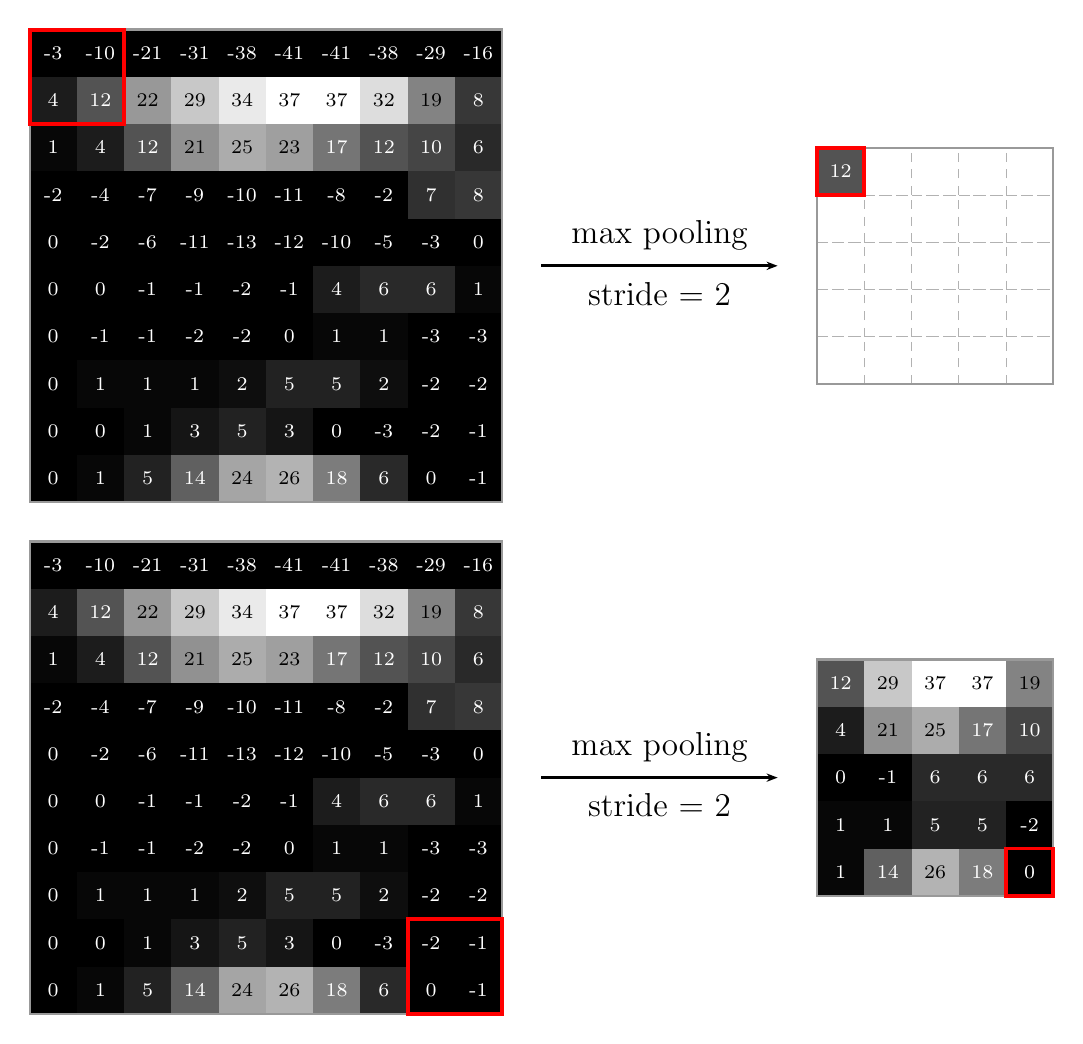
\begin{tikzpicture}[>={Stealth[length=4pt]}, line width=0.8pt, font=\large]

  % ========== 可复用：NxN 灰度图（全填充，#1 = 宽度 N） ==========
  \newcommand{\drawresultfull}[4]{%
    \foreach \v [count=\n] in {#4} {%
      \pgfmathtruncatemacro{\r}{int((\n-1)/#1)}
      \pgfmathtruncatemacro{\c}{int(mod(\n-1,#1))}
      \pgfmathsetmacro{\g}{max(0, min(\v/37, 1))}
      \definecolor{oc}{gray}{\g}
      \ifdim\g pt>0.5pt \def\tc{black}\else \def\tc{white}\fi
      \fill[oc] ({#2+0.6*\c}, {#3+0.6*(#1-1-\r)}) rectangle ++(0.6,0.6);
      \node[font=\scriptsize, text=\tc] at ({#2+0.6*\c+0.3}, {#3+0.6*(#1-1-\r)+0.3}) {\v};
    }%
    \draw[gray!80] (#2,#3) rectangle ({#2+0.6*#1}, {#3+0.6*#1});
  }

  % ================= 第一行：左上角 2x2 -> 第一个池化值（不变） =================
  \drawresultfull{10}{0}{7}{%
    -3,-10,-21,-31,-38,-41,-41,-38,-29,-16,%
    4,12,22,29,34,37,37,32,19,8,%
    1,4,12,21,25,23,17,12,10,6,%
    -2,-4,-7,-9,-10,-11,-8,-2,7,8,%
    0,-2,-6,-11,-13,-12,-10,-5,-3,0,%
    0,0,-1,-1,-2,-1,4,6,6,1,%
    0,-1,-1,-2,-2,0,1,1,-3,-3,%
    0,1,1,1,2,5,5,2,-2,-2,%
    0,0,1,3,5,3,0,-3,-2,-1,%
    0,1,5,14,24,26,18,6,0,-1}
  \draw[red, line width=1.4pt] (0,11.8) rectangle (1.2,13);    % 左上 2x2
  \draw[->, line width=1pt] (6.5,10) -- (9.5,10)
    node[midway, above=2pt] {max pooling}
    node[midway, below=2pt] {stride = 2};
  % 右边 5x5：只有左上角有值，其余虚线
  \foreach \r in {0,...,4} \foreach \c in {0,...,4}
    \draw[gray!60, dashed, line width=0.3pt] ({10+0.6*\c}, {8.5+0.6*\r}) rectangle ++(0.6,0.6);
  \pgfmathsetmacro{\g}{12/37}
  \definecolor{oc}{gray}{\g}
  \fill[oc] (10,10.9) rectangle (10.6,11.5);
  \node[font=\scriptsize, text=white] at (10.3,11.2) {12};
  \draw[gray!80] (10,8.5) rectangle (13,11.5);
  \draw[red, line width=1.4pt] (10,10.9) rectangle (10.6,11.5);  % 对应左上角

  % ================= 第二行：右下角 2x2 -> 最后一个池化值（★ 整体上移 0.5） =================
  \drawresultfull{10}{0}{0.5}{%
    -3,-10,-21,-31,-38,-41,-41,-38,-29,-16,%
    4,12,22,29,34,37,37,32,19,8,%
    1,4,12,21,25,23,17,12,10,6,%
    -2,-4,-7,-9,-10,-11,-8,-2,7,8,%
    0,-2,-6,-11,-13,-12,-10,-5,-3,0,%
    0,0,-1,-1,-2,-1,4,6,6,1,%
    0,-1,-1,-2,-2,0,1,1,-3,-3,%
    0,1,1,1,2,5,5,2,-2,-2,%
    0,0,1,3,5,3,0,-3,-2,-1,%
    0,1,5,14,24,26,18,6,0,-1}
  \draw[red, line width=1.4pt] (4.8,0.5) rectangle (6,1.7);      % 右下 2x2
  \draw[->, line width=1pt] (6.5,3.5) -- (9.5,3.5)
    node[midway, above=2pt] {max pooling}
    node[midway, below=2pt] {stride = 2};
  % 右边 5x5 全算完
  \drawresultfull{5}{10}{2.0}{%
    12,29,37,37,19,%
    4,21,25,17,10,%
    0,-1,6,6,6,%
    1,1,5,5,-2,%
    1,14,26,18,0}
  \draw[red, line width=1.4pt] (12.4,2.0) rectangle (13,2.6);  % 对应右下角
\end{tikzpicture}
\end{document}